\chapter{Spectroscopy - Exploring Emission \& Absorption}
\thispagestyle{fancy}
\fancyhead[RE,LO]{Experiment \thechapter}
%
\begin{wrapfigure}{R}{0.50\textwidth}
  \vspace{-25pt}  
  \begin{center}
    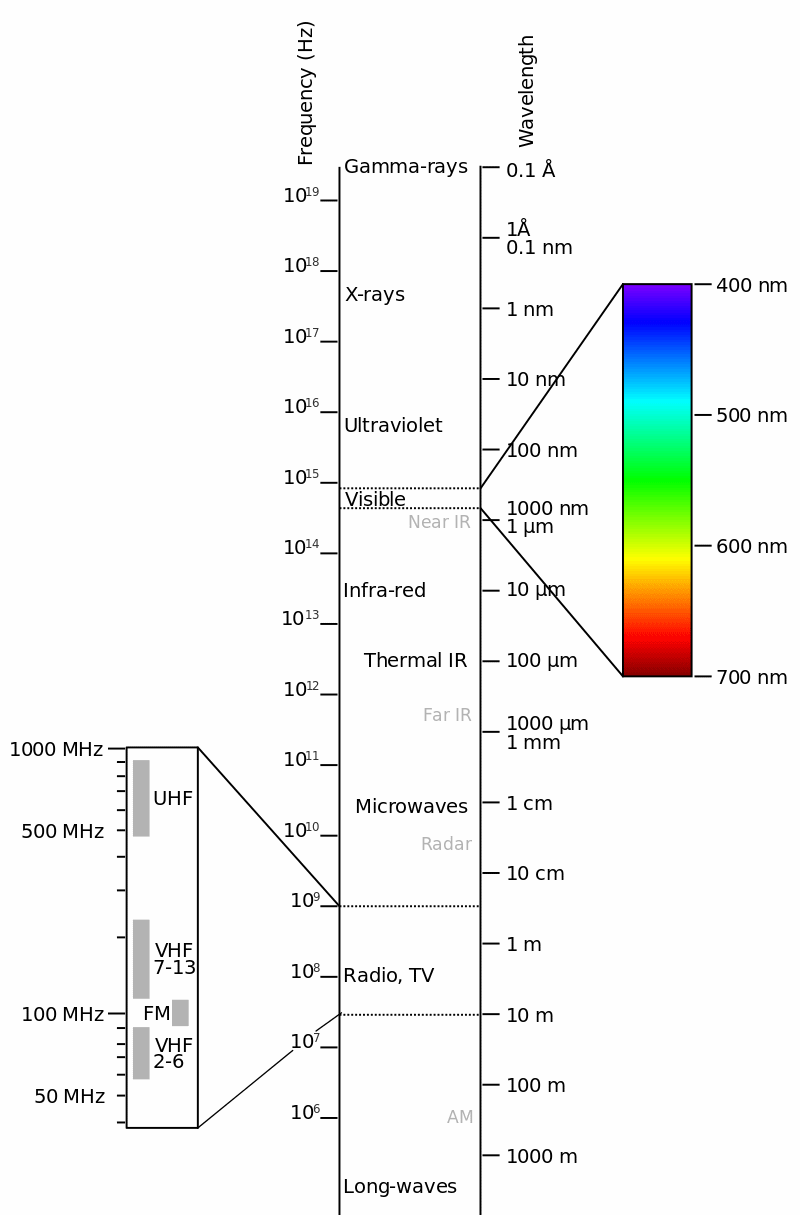
\includegraphics[width=0.48\textwidth]{emSpectrum}
  \end{center}
  \caption{The electromagnetic spectrum.}
  \label{fig:emSpec}
  \vspace{-5pt}
\end{wrapfigure}
In this two-week lab, we will be exploring the interaction of light with matter. 
Using spectroscopy (also called spectral analysis, spectrometry, or spectrophotometry), we will examine emission and absorption of light by various substances. 
Spectroscopes (also called spectrometers and spectrophotometers) are measurement tools designed to distinguish different colors of light. 
The spectrometers we will use in this lab detect the intensity of the light (the power-per-area associated with the light) as a function of the wavelength of the light. 
These spectrometers have a sensitivity range from 350 nm to 1000 nm, with a spectral resolution of 2 nm. 
In contrast, the human eye has a sensitivity range from approximately 400 nm (violet) to 700 nm (red), with a spectral resolution ranging from 1 nm (in the green to yellow range) to 10 nm (in the violet and red ranges). 
You may have been exposed to spectroscopy data through your previous chemistry and biology courses. 
To thoroughly understand data, one must know where it came from, its limitations, and its interpretations and potential meanings. 
With this lab we hope to deepen your comprehension of the function of spectrometers and thereby enrich your understanding of the data they produce. 
This will lay a firm foundation for your use of spectroscopy in your broader scientific career. 
\par
Matter has rich internal activity. 
Since matter is bound together in stable situations by forces, it has lots of natural ways to oscillate and resonate. 
The methyl groups on organic molecules can spin around. 
Similarly, long molecular chains can vibrate back-and-forth like a spring. 
Within each atom, electrons are constantly shifting towards and away from the nucleus. 
Each of these processes has a particular wavelength (color) of light associated with it: a specifically-sized photon energy packet is emitted or absorbed. 
Since light can only be absorbed or emitted in these packets, the way different colors of light interact with matter tells us about the energy spacing between the allowed excitation states of atoms and molecules. 
Doing a spectral analysis of light emitted or absorbed by something can give us a lot of information about it. 
Stokes (famous for his study of viscosity) was the first to show that hemoglobin was the molecule responsible for carrying oxygen in the blood—he did this using spectral analysis! 
On an entirely different physical scale, it's spectral analysis that permits us to figure out the composition of stars. 

\subsection*{A Short Introduction to Light/Quantization:}
The range of all possible light waves is referred to as the Electromagnetic (EM) Spectrum (see figure~\ref{fig:emSpec}). 
Of this range, the 'visible' portion (sensed by the human eye, $\sim$400nm - 700nm) is only a very small section. 
These waves move at a speed of $c = 3.0 \times 10^{8} \: m/s$ in a vacuum. 
Their frequency, $f$, and wavelength, $\lambda$, are related with their speed, $v$, according to: $v = f \lambda$. 
The energy, $E$, carried by these waves is proportional to their frequency: $E = h f$, where the proportionality constant, $h$, is Planck's constant ($h = 6.63 \times 10^{-34} \; kg \, m^{2}/s$). 
\par
All of these different waves are produced by electric charges moving, oscillating, and resonating in very specific ways. 
For each resonant frequency producing a photon of light there is an associated packet of energy, called a quantum. 
Because all light is made of these packets, these quanta, we say that light is quantized.

\paragraph{For this two week lab:} Your lab will consist of three parts: I) exploring the quantized atom; II) exploring emission and absorption; and III) considering the evolutionary adaptation of the visible spectrum of the human eye. 
The lab report you turn in at the end of the second week should discuss answers to questions posed in the sections below as well as any insights you gain from your explorations and investigations, along with the data supporting those insights.
You will do this in multiple stages:
\begin{enumerate}
\itemsep-0.2em
\item Get familiar with the equipment.
\item Capture emission spectra from all the available light sources.
\end{enumerate}

\newpage

\section*{About the Equipment:}
Each group has access to:
\begin{itemize}
\itemsep-0.3em
\item a spectrometer and fiber optic cable that can interface with the computer via the USB,
\item Logger Pro software for the computer,
\item a small stand with multiple 90-clamps,
\item a long pole with table clamp,
\item an assortment of filters/cards, including Green, Red, Yellow, and UV filters and a diffraction grating,
\item a variety of hand-held diffraction grating spectrometers,
\item a classroom set of light sources/lamps: H, Na, Hg, and UV,
\item small LED light boxes emitting different colors of light (Red, Green, and Blue),
\item a light ray box (with an incandescent bulb that acts as a white light source),
\item a meter stick, and
\item an aquarium (fish tank) that can be filled with water.
\end{itemize}
BE GENTLE WITH THE EQUIPMENT!! 
Handle all heavy equipment with care. 
Watch out for all of the wires and cables. 
Keep all fluids away from the computer and spectrometer.
You may be operating in low light conditions, so proceed with caution. 
The Na and Hg lamps will need to warm-up before they produce a usable spectrum. 
Masking the light ray box will help reduce glare from reflections (ask your TA/LA for help with this). 
You may find it helpful to use the fiber optic sensor in conjunction with a fixed holder/mount.

\section*{Part I: Exploring the Quantized Atom}
%
\begin{wrapfigure}{R}{0.44\textwidth}
  \vspace{-15pt}  
  \begin{center}
    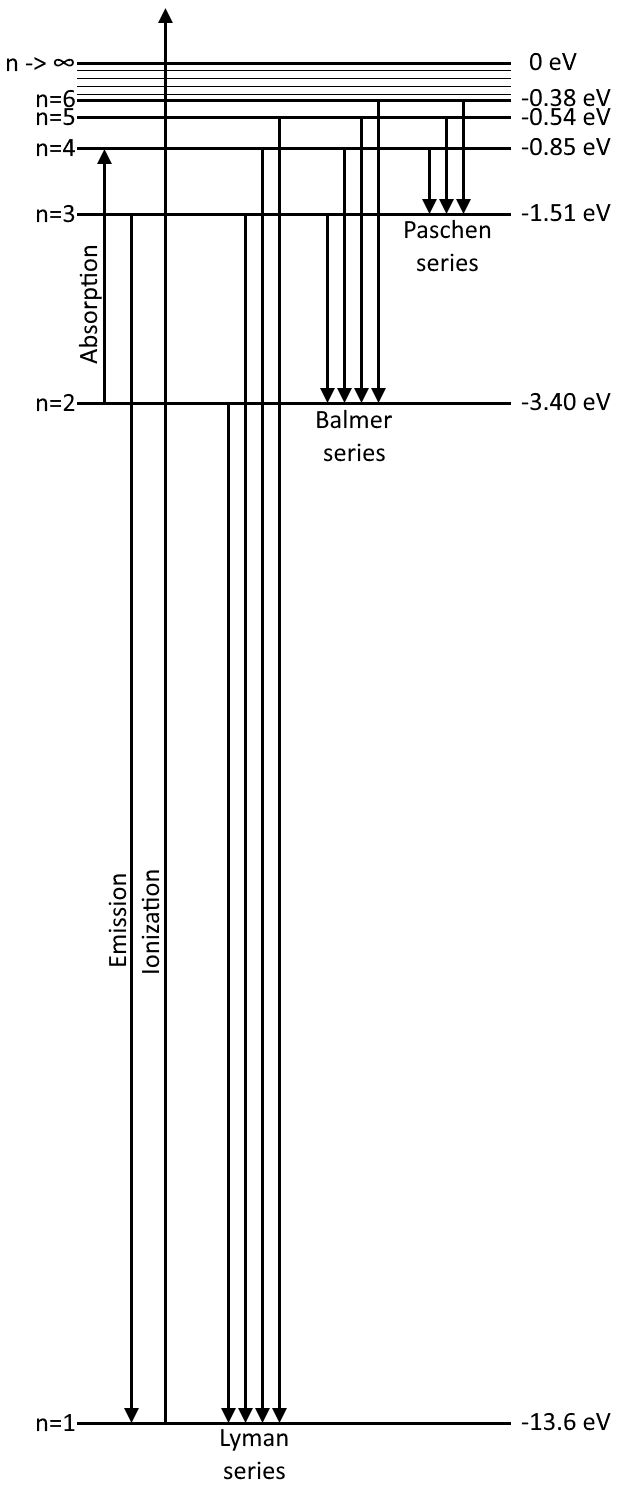
\includegraphics[width=0.42\textwidth]{energy_levels}
  \end{center}
  \vspace{-20pt}
  \caption{Energy level transitions for the Bohr Model of the hydrogen atom.}
  \label{fig:e-levels}
  \vspace{-10pt}
\end{wrapfigure}
%
Perhaps the most 'illuminating' model of the quantization of light is the Bohr model of the hydrogen (H) atom. 
In this model, the proton nucleus of the hydrogen atom is orbited by the single electron at fixed orbital radii. 
When the atom is excited (absorbs energy), the electron transitions from the ground state (lowest energy level) to an excited state. 
The electron will then transition back to a lower energy state, emitting this energy difference between levels as a photon of light. 
The Bohr model is a good model for explaining why only certain frequencies/wavelengths of light are absorbed or emitted by an atom. 
It also explains the Rydberg formula for the emission lines of the hydrogen spectrum—this formula was well-established experimentally as early as 1888, but had no theoretical explanation until the Bohr model was introduced in 1913 (25 years later!). 
\par 
Some of the energy level transitions within the hydrogen atom have been given specific names. 
All transitions to/from the ground state (lowest energy level, $n = 1$) are part of the Lyman series. 
All transitions to/from the 1st excited stated ($n = 2$) are part of the Balmer series. 
All transitions to/from the 2nd excited state ($n = 3$) are part of the Paschen series. 
Other transitions also have formal names, but the Lyman, Balmer, and Paschen are the most commonly encountered. 
Each level (each $n$) has an associated energy given by: $E_{n}=(-13.606 eV)/(n^{2})$. 
(Recall that 1 Joule $= 6.2415 \times 10^{18} eV$.) 
\par 
Figure~\ref{fig:e-levels} shows the energy levels for the Bohr model of the hydrogen atom and the associated energy level transitions. 
How are these similar? 
How are they different? 
Are any of the charts communicating the information in more helpful/clear ways? 
Are any of the charts misleading in the communication of information? 
Which chart does your group like best?
\par
We would like to know which of these series is observed in the hydrogen emission spectrum.
Using the hydrogen lamp (ask the TA/LA if you need help identifying this lamp) and the spectrometer with fiber optic cable, collect data for the emission spectrum of hydrogen. 
To collect the data with Logger Pro, open the My Documents folder on your Desktop and double-click on “Spectrometer.cmbl.” 
Clicking on the green "Collect" button will enable you to gather information.
Direct the end of the fiber optic cable toward your light source (the pin-hole on the end of the cable is where the light enters — it is sensitive to direction and distance from source, so keep these considerations in mind). 
To keep the data, click "Stop." 
When you wish to gather another data set, click "Collect" — you can overwrite the previous data set OR you can keep the old data and display the new data as well as the old data (choose "Store Latest Run"). 
To get rid of a stored data set, choose Data $>$ Delete Data Set and select the appropriate set for deletion. 
When you have a good, clean, clear emission spectrum for the hydrogen lamp, print out your emission spectrum graph (of power vs. wavelength).
\par 
Which wavelengths are present in the hydrogen emission spectrum? 
Do these transitions represent the Lyman, Balmer, or Paschen series? 
Justify your claim by comparing your data to the Bohr model. 
\par 
As noted earlier, the Bohr model gave a theoretical reasoning for a long-standing experimental result. 
The Rydberg formula for the hydrogen emission spectrum is written below. 
Using your data, find the Rydberg constant, R. 
What is the range of uncertainty for your value of R?
\vfill
\noindent
Rydberg formula for hydrogen:
\[ \frac{1}{\lambda_{vac}} = R \left( \frac{1}{n_{1}^{2}} - \frac{1}{n_{2}^{2}} \right) \]
where $ \lambda_{vac} $ is the wavelength of electromagnetic radiation emitted in a vacuum, $R$ is the Rydberg constant ($R = 1.09678\times 10^{-2} \: nm^{-1}$), and $n_{1}$ and $n_{2}$ are integers greater than or equal to 1, such that $n_{1} < n_{2}$.

\section*{Part II: Exploring Emission and Absorption}
Now let’s investigate emission of light by different sources and the ways in which absorption affects the recorded spectra. 
You can use the hand-held diffraction grating spectrometers (you have three types of these) and the diffraction grating card to get a qualitative sense of the spectra produced by different sources (including the sun light from the window and the fluorescent lights in the ceiling). 
If using the spectrometer and fiber optic cable will help you describe your sources more accurately, feel free to use this, too. 
Try different combinations of sources and filters. 
Your task in this portion of the lab is to develop an understanding of what spectra are produced by different sources and how these spectra compare and contrast. 
Additionally, you should develop an understanding of how absorption (by glass, water, various filters, solid-colored surfaces, etc.) affects the transmitted spectrum. 
There is a lot of different equipment involved in these investigations, so let's rotate ourselves to different tables (rather than shifting the equipment between tables). 
Remember to take notes on the observations and insights you gain from your investigations. 
To aid you in this exploration, you might consider the following questions (these are suggested, but not mandated):
\begin{itemize}
\itemsep-0.3em
\item How do the various filters change the spectrum produced by the hydrogen lamp?
\item What does a ‘red’ filter do?
\item How are the spectra produced by the sodium (Na) or mercury (Hg) lamps similar to and different from that produced by the hydrogen (H) lamp?
\item How is the sun’s spectrum different from or similar to those produced by the lamps (H, Na, and Hg)? Is the sun’s spectrum still ‘quantized’? Why or why not?
\item Is the sun’s spectrum the same outside the window as it is when the sun has travelled through the window’s glass? (Does the glass absorb any light? If so, which frequencies or bands of frequencies are most affected?)
\item What do you see when you look at an incandescent (heated filament) source, such as the bulb in the light ray box? How does this spectrum compare to the sun’s?
\item How do the UV (ultra-violet) and LED light sources compare to the solar spectrum or to the incandescent spectrum? How do the filters change the spectra observed from these sources?
\item Does water act as a filter? If so, which frequencies or bands of frequencies are most affected?
\item What factors affect the observed color of different reflective surfaces (like your t-shirts or your notebook covers)?
\item What effect do combinations of filters have on observed spectra?
\item What frequencies or bands of frequencies are affected by using your sunglasses as a filter? Are all sunglasses the same?
\item How does the distance of the fiber optic sensor from the source affect the observed spectra?
\end{itemize}
Before you move on to Part III, consider what mechanisms inside the spectrometer (with the fiber optic cable) enable it to detect different wavelengths of light. 
What are the physical mechanisms within this ‘black box’ measurement tool? 
Discuss this as part of your lab report.

\section*{Part III: Considering the Evolutionary Adaptation of the Visible Spectrum of the Human Eye}
The mechanisms by which living creatures `see' the world around them vary significantly across species. 
Even more remarkably, this diversity of evolutionary adaptations exists even though all living things were exposed to the same ultimate source: the sun. 
The solar spectrum is, in fact, very different from the spectrum to which the human eye is sensitive (often called the ‘Visible’ spectrum). 
Many insects and some birds are sensitive to wavelengths, particularly in the ultraviolet, that are completely invisible to the human eye; thus, the visible spectrum of a bee or a bird can be quite different from that of a human. 
Bees, birds, turtles, lizards, many fish and some rodents have UV receptors in their retinas. 
These animals can see the UV patterns found on flowers and other wildlife that are otherwise invisible to the human eye. 
The schlieren photograph (at left) shows the zones of a fish lens that focus different spectral ranges (red on the outside edge, toward UV at the center). 
Some animals, such as reptiles (e.g. snakes), have IR (infra-red) sensitivity. 
\par 
Why have humans developed eyes sensitive only to the Visible spectrum (~400 nm – 700 nm)? 
Why are the UV and IR bands, present in the solar spectrum and in the visible spectra of other living creatures, absent from the visible spectrum of the human eye? 
Your task is to develop plausible hypotheses for the evolutionary adaptations resulting in the absence of UV and IR sensitivity in the human eye and to collect spectral data to support the plausibility of your hypotheses. 
The following two charts may (or may not!) help you get started in thinking about plausible hypotheses.

\section*{For your report:}
The lab write-up should include careful discussions of (a) your insights and investigations for Parts I and II, (b) discussions of any data that support these insights, (c) your investigations into the evolutionary adaptation of the visible spectrum of the human eye (Part III), and (d) your comparison of your work with the work of other groups, as well as your critique of your experiment and conclusions. 
If you want to include hand-drawn elements (such as ray diagrams), please do so. 
Please also consider what is going on inside the spectrometer connected to the USB/computer. 
Discuss the physical mechanisms inside this `black box'.